\documentclass[rgb]{beamer}

\usepackage[english]{babel}
\usepackage[utf8]{inputenc}
\usepackage{xcolor}
\usepackage{listings}
\usepackage{adjustbox}
\usepackage{amsmath}
\usepackage{multirow}
\usepackage[linewidth=1pt]{mdframed}

% Graphics
\usepackage{graphicx}

\usepackage{tikz}
\usetikzlibrary{calc,shapes.multipart,chains,arrows}

% Font
\usepackage{paratype}
\setbeamerfont{frametitle}{family=\bf}

% Beamer theme settings
\usecolortheme{seagull}
\setbeamertemplate{itemize item}{\raisebox{0.8mm}{\rule{1.8mm}{1.2mm}}}
\usenavigationsymbolstemplate{} % no navigation buttons

\usepackage{listings}

% Define Language
\lstdefinelanguage{fsharp}
{
  % list of keywords
  morekeywords={
    and,
    do,
    else,
    exception,
    for,
    fun,
    function,
    if,
    in,
    let,
    match,
    module,
    mutable,
    open,
    of,
    rec,
    then,
    try,
    type,
    unsafe,
    use,
    val,
    when,
    while,
    with,
  },
  sensitive=true, % keywords are not case-sensitive
  morecomment=[l]{//}, % l is for line comment
%  otherkeywords={>,<,=,<=,>=,!,*,/,-,+,|,&,||,&&,==,=>},
  morestring=[b]" % defines that strings are enclosed in double quotes
}

% Define Colors
\usepackage{color}
\definecolor{eclipseBlue}{RGB}{42,0.0,255}
\definecolor{eclipseGreen}{RGB}{63,127,95}
\definecolor{eclipsePurple}{RGB}{127,0,85}

\newcommand{\fop}[1]{\mbox{\ttfamily\color{eclipseBlue}#1}}
\newcommand{\fw}[1]{\mbox{\ttfamily\bfseries\color{eclipsePurple}#1}}

% Set Language
\lstset{
  language={fsharp},
  basicstyle=\ttfamily, % Global Code Style
  captionpos=b, % Position of the Caption (t for top, b for bottom)
  extendedchars=true, % Allows 256 instead of 128 ASCII characters
  tabsize=2, % number of spaces indented when discovering a tab
  columns=fixed, % make all characters equal width
  keepspaces=true, % does not ignore spaces to fit width, convert tabs to spaces
  showstringspaces=false, % lets spaces in strings appear as real spaces
  breaklines=true, % wrap lines if they don't fit
  frame=trbl, % draw a frame at the top, right, left and bottom of the listing
  frameround=tttt, % make the frame round at all four corners
  framesep=4pt, % quarter circle size of the round corners
  numbers=left, % show line numbers at the left
  numberstyle=\small\ttfamily, % style of the line numbers
  commentstyle=\slshape\bfseries\color{eclipseGreen}, % style of comments
  keywordstyle=\bfseries\color{eclipsePurple}, % style of keywords
  stringstyle=\color{eclipseBlue}, % style of strings
  emph=[1] {
    false,
    true,
    Set,
    Map,
    List,
    ImgUtil,
    Pegs,
    String,
    Array,
    Array2D
  },
  emphstyle=[1]{\color{eclipseBlue}},
  moredelim=**[is][\color{red}]{@@}{@@}
}

\newcommand{\theyear}{2020}
\newcommand{\sem}[1]{[\![#1]\!]}
\newcommand{\seme}[1]{\sem{#1}\varepsilon}
\newcommand{\semzero}[1]{\sem{#1}_0}

\newcommand{\emptymap}{\{\}}
\newcommand{\fracc}[2]{\begin{eqnarray} \frac{\begin{array}{c} #1
    \end{array}}{\begin{array}{c} #2 \end{array}} \end{eqnarray}}
\newcommand{\sembox}[1]{\hfill \normalfont \mbox{\fbox{\(#1\)}}}
\newcommand{\sempart}[2]{\subsubsection*{\rm\em #1 \sembox{#2}}}
\newcommand{\axiom}[1]{\begin{eqnarray} \begin{array}{c} #1 \end{array} \end{eqnarray}}
\newcommand{\fraccn}[2]{\refstepcounter{equation}\mbox{$\frac{\begin{array}{c} #1 \end{array}}{\begin{array}{c} #2 \end{array}}$}~(\arabic{equation})}
\newcommand{\fraccc}[2]{\mbox{$\frac{\begin{array}{c} #1 \end{array}}{\begin{array}{c} #2 \end{array}}$}}
\newcommand{\onepart}[1]{\noindent\hfill#1\hfill~\vspace{2mm}}
\newcommand{\twopart}[2]{\noindent\hfill#1\hfill#2\hfill~\vspace{2mm}}
\newcommand{\threepart}[3]{\noindent\hfill#1\hfill#2\hfill#3\hfill~\vspace{2mm}}
%\newcommand{\axiomm}[1]{\refstepcounter{equation}\mbox{$\begin{array}{c} #1 \end{array}$}~(\arabic{equation})}
\newcommand{\axiomm}[1]{$\begin{array}{c} #1 \end{array}$}
%\newcommand{\ar}[1]{\stackrel{#1}{\longrightarrow}}
\newcommand{\vd}{\vdash}
\newcommand{\Ran}{{\rm Ran}}
\newcommand{\Dom}{{\rm Dom}}
\newcommand{\kw}[1]{\texttt{#1}}
\newcommand{\id}[1]{\mbox{\it{#1}}}
\newcommand{\rarr}{\rightarrow}
\newcommand{\eval}{\rarr}
\newcommand{\evals}{\leadsto}
\newcommand{\larr}{\leftarrow}

\newcommand{\head}[1]{\vspace{3mm} \textbf{\normalsize #1}}
\newcommand{\headsp}[1]{\head{#1}\vspace{1ex}}
\newcommand{\size}{\ensuremath{\mathrm{size}}}
\renewcommand{\log}{\ensuremath{\mathrm{log}}}

\newcommand{\setallthemecolors}[1]{%
\setbeamercolor*{palette primary}{use=structure,fg=white,bg=#1}%
\setbeamercolor*{palette secondary}{use=structure,fg=white,bg=#1}%
\setbeamercolor*{palette tertiary}{use=structure,fg=white,bg=#1}}

\definecolor{black}{RGB}{0,0,0}
\definecolor{maroon}{RGB}{128,0,0}
\definecolor{olive}{RGB}{128,128,0}
\definecolor{green}{RGB}{0,128,0}
\definecolor{purple}{RGB}{128,0,128}
\definecolor{teal}{RGB}{0,128,128}
\definecolor{darkteal}{RGB}{0,92,92}
\definecolor{navy}{RGB}{0,0,128}
\definecolor{gray}{RGB}{128,128,128}
\definecolor{darkgray}{RGB}{60,60,60}
\definecolor{darkred}{RGB}{139,0,0}

%palette

% #173F5F (dark blue)
\definecolor{darkblue}{RGB}{23,63,95}
% #20639B (blue)
\definecolor{blue}{RGB}{32,99,155}
% #3CAEA3 (green)
\definecolor{magenta}{RGB}{60,174,163}
% #F6D55C (yellow)
\definecolor{yellow}{RGB}{246,213,92}
% #ED553B (red)
\definecolor{red}{RGB}{237,85,59}


\usecolortheme{whale}
\useoutertheme{infolines}
\useinnertheme{rectangles}

\newcommand{\popsettitle}[2]{%
\setallthemecolors{#1}%
\newcommand{\popemne}{#2}%
\title{Programmering og Problemløsning}%
\subtitle{#2}%
\author{Martin Elsman}%
\date{}%
\institute[DIKU]{Datalogisk Institut, Københavns Universitet (DIKU)}}

\newcommand{\popmaketitleframe}{%
  \frame{\titlepage%
   \vspace{-15mm}%
   \par\noindent\rule{\textwidth}{0.4pt}%

   \vspace{4mm}%
   \tableofcontents%
   \vspace{-4mm}%
   \par\noindent\rule{\textwidth}{0.4pt}%
  }%
  \section*{\popemne}%
}


\popsettitle{blue}{Rekursion (Del 4)}  % see ../util.tex for colors

\begin{document}

\popmaketitleframe

%%%%%%%%%%%%%%%%%%%%%%%%%%%%%%%%%%%%%%%%%%%%%%%%
\subsection{Funktionsprogrammering contra imperativ programmering}
%%%%%%%%%%%%%%%%%%%%%%%%%%%%%%%%%%%%%%%%%%%%%%%%

\begin{frame}[fragile]
\begin{footnotesize}

  \headsp{Funktionstyper og funktionsprogrammering}

  \vspace{2mm}
  \textbf{Q1:} Hvorfor beskæftiger vi os overhovedet med typer?
  \vspace{1mm}

  \begin{itemize}
  \item \underline{\hspace{10cm}}
% For at beskrive de datastrukturer (værdier) vores programmer arbejder på
  \end{itemize}

  \vspace{2mm}
  \textbf{Q2:} Hvad beskriver funktionstypen \lstinline{int->int}
  \vspace{1mm}

  \begin{itemize}
  \item \underline{\hspace{10cm}}
% Funktioner der tager et heltal som argument og returnerer et heltal
  \end{itemize}

  \vspace{2mm}
  \textbf{Q3:} I den kontekst, hvad er forskellen på værdiorienteret (funktionel) programmering og effektfuld (imperativ) programmering?
  \vspace{1mm}

  \begin{itemize}
  \item \underline{\hspace{10cm}}
% Funktionelle programmer har ingen ``sideeffekter''
  \end{itemize}

  \vspace{2mm}
  \textbf{Q4:} Beskriv forskellen på typerne \lstinline{int*int->int} og \lstinline{int->int->int}
  \vspace{1mm}

  \begin{itemize}
  \item \underline{\hspace{10cm}}
% a) beskriver funktioner der tager et par som argument og returnerer et heltal mens b) beskriver funktioner der tager et heltal som argument og returnerer en funktion
  \end{itemize}

  \vspace{2mm}
  \textbf{Q5:} Beskriv forskellen på typerne \lstinline{int->int->int} og \lstinline{(int->int)->int}
  \vspace{1mm}

  \begin{itemize}
  \item \underline{\hspace{10cm}}
% b) beskriver funktioner der tager en funktion som argument of returnerer et heltal
  \end{itemize}

\end{footnotesize}
\end{frame}

\begin{frame}[fragile]
\begin{footnotesize}

  \headsp{Hvorfor typer?}

  \vspace{3mm}
  \begin{quote}
    \emph{"Show me your flowchart and conceal your tables, and I shall continue to be mystified. Show me your tables, and I won't usually need your flowchart; it'll be obvious."} --- Fred Brooks, The Mythical Man Month (1975)
  \end{quote}

  \vspace{3mm}
  \begin{quote}
    \emph{"Bad programmers worry about the code. Good programmers worry about data structures and their relationships."} --- Linus Torvalds
  \end{quote}


  \vspace{3mm}
  \begin{itemize}
  \item Typer beskriver data.
  \item Typer kan bruges ifbm design af programmer / funktioner.
  \item Vi kan statisk (ved oversættelse) verificere at en
    værdi er af en given type.
  \item Typer giver os udtrykskraft!
  \item ...
  \end{itemize}
\end{footnotesize}
\end{frame}

%%%%%%%%%%%%%%%%%%%%%%%%%%%%%%%%%%%%%%%%%%%%%%%%
\subsection{Rekursion (Recap)}
%%%%%%%%%%%%%%%%%%%%%%%%%%%%%%%%%%%%%%%%%%%%%%%%

\begin{frame}[fragile]

  \headsp{Rekursion over heltal}

  \headsp{Halerekursion}

  \headsp{Rekursion over lister med pattern-matching}

  \begin{minipage}[t]{.7\textwidth}
  \begin{itemize}
  \item Mergesort
  \end{itemize}
  \end{minipage}
  \begin{minipage}{.25\textwidth}
  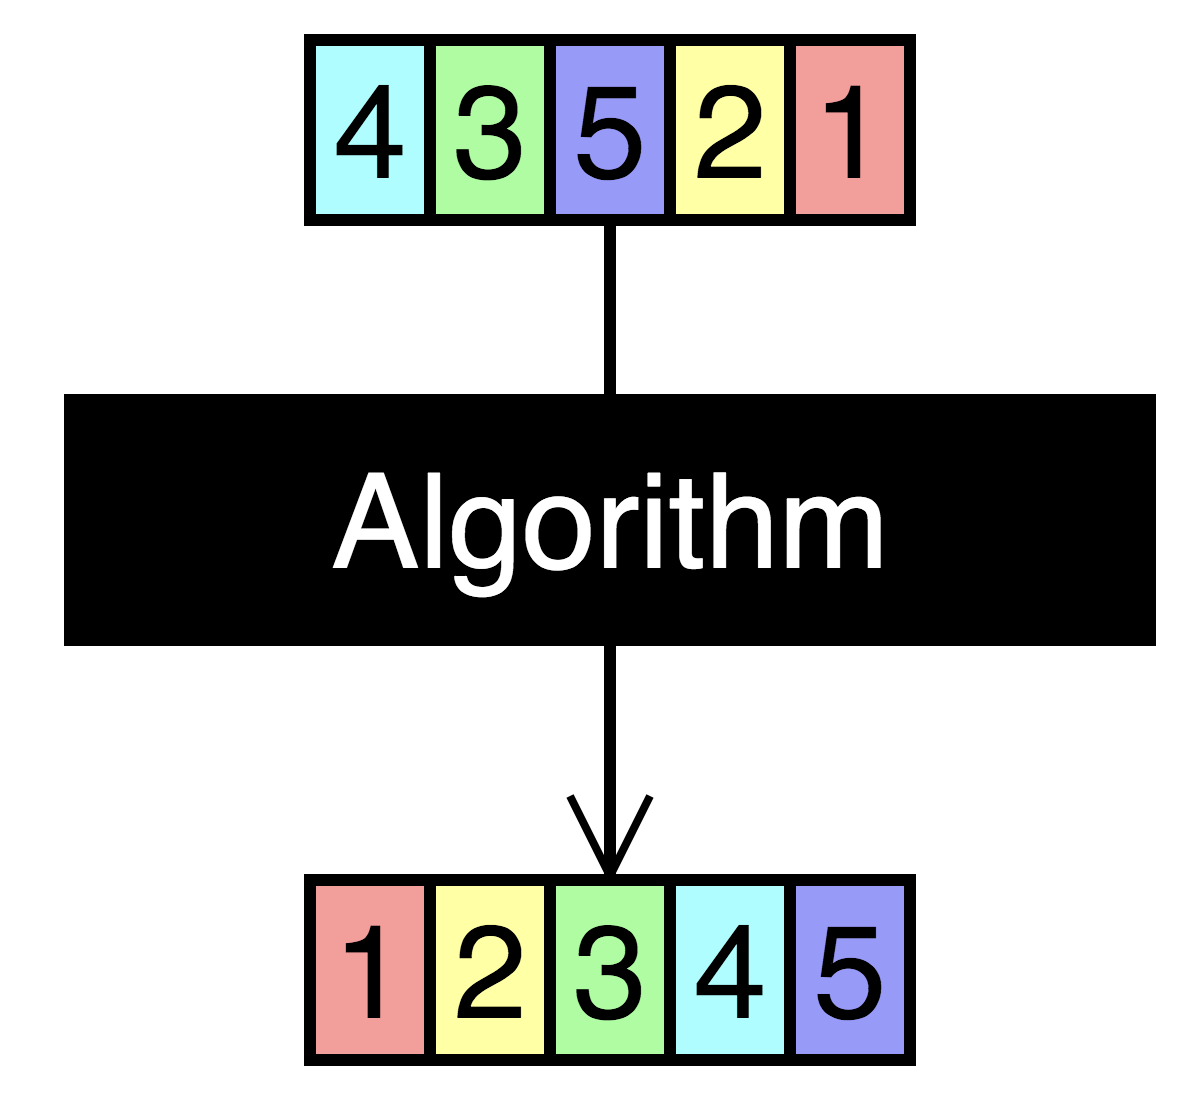
\includegraphics[width=\textwidth]{../images/sorting_algorithms.png}
  \end{minipage}
\end{frame}

\begin{frame}[fragile]
\begin{footnotesize}

\headsp{Rekursion over heltal}

\begin{lstlisting}[numbers=none,frame=none,mathescape]
let rec count (n:int64) : int64 =
  if n <= 0L then 0L
  else 1L + count (n-1L)

let x = count 100000L   // ok
let y = count 1000000L  // stack overflow
\end{lstlisting}

\vspace{2mm}
\headsp{Halerekursion}

\begin{lstlisting}[numbers=none,frame=none,mathescape]
let rec hcount (a:int64) (n:int64) : int64 =
  if n <= 0L then a
  else hcount (a+1L) (n-1L)

let count = hcount 0L      // delvis funktions-anvendelse!

let x = count 100000L      // ok
let y = count 1000000000L  // ok
\end{lstlisting}

\end{footnotesize}
\end{frame}

\begin{frame}[fragile]
\begin{footnotesize}

  \head{Mergesort --- divide-and-conquer (del-og-hersk!)}

  \emph{John von Neumann, 1945}

  \begin{itemize}
  \item Opdel listen i to lige store dele.
  \item Sort\'er (rekursivt) hver liste.
  \item Flet (merge) de to resultater.
  \end{itemize}

  \head{En implementation i F\#:}

\begin{lstlisting}[numbers=none,frame=none,mathescape]
let rec msort xs =
  let sz = List.length xs
  if sz < 2 then xs
  else let n = sz / 2
       let ys = xs.[0..n-1]
       let zs = xs.[n..sz-1]
       in merge (msort ys) (msort zs)
\end{lstlisting}

\head{Bemærk:}
\begin{itemize}
\item Mergesort benytter sig af slice-syntaksen (e.g., \lstinline{xs.[0..n-1]}) for at udtrække dele af en liste.
\item Mergesort benytter sig af utility-funktionen \lstinline{merge} (next slide).
\end{itemize}
\end{footnotesize}
\end{frame}

\begin{frame}[fragile]
\begin{footnotesize}
\head{Utility-funktionen \lstinline{merge}}

\vspace{1ex}

\begin{lstlisting}[numbers=none,frame=none,mathescape]
let rec merge xs ys =
  match xs, ys with    // pattern-matching par
    | [], _ -> ys      // af lister!
    | _, [] -> xs
    | x::xs, y::ys -> if x<y then x::merge xs (y::ys)
                      else y::merge (x::xs) ys
\end{lstlisting}

\head{Bemærk:}
\begin{itemize}
\item Funktionen \lstinline{merge} fletter to sorterede lister sammen således at resultatet er sorteret.
\item Vi skal senere se på pattern-matching generelt...
\end{itemize}

\end{footnotesize}
\end{frame}

\begin{frame}[fragile]
\begin{footnotesize}
\head{Analyse af Mergesort}

\vspace{1ex}

\begin{minipage}[b]{0.55\textwidth}

  Kald-træet for \lstinline{msort} er $\log(N)$ dybt og
  \lstinline{merge} kaldes i hver knude. Det viser sig at Best time =
  Worst time = Average time = $O(N\log(N))$.

\vspace{1ex}

\head{Summary:}

\vspace{1ex}
  \begin{tabular}{ll}
    Best time: & $O(N\log(N))$ \\
    Worst time: & $O(N\log(N))$ \\
    Average time: & $O(N\log(N))$
  \end{tabular}

  \vfill
\mbox{ }
\end{minipage} \hspace{1cm}
\begin{minipage}[b]{0.3\textwidth}

  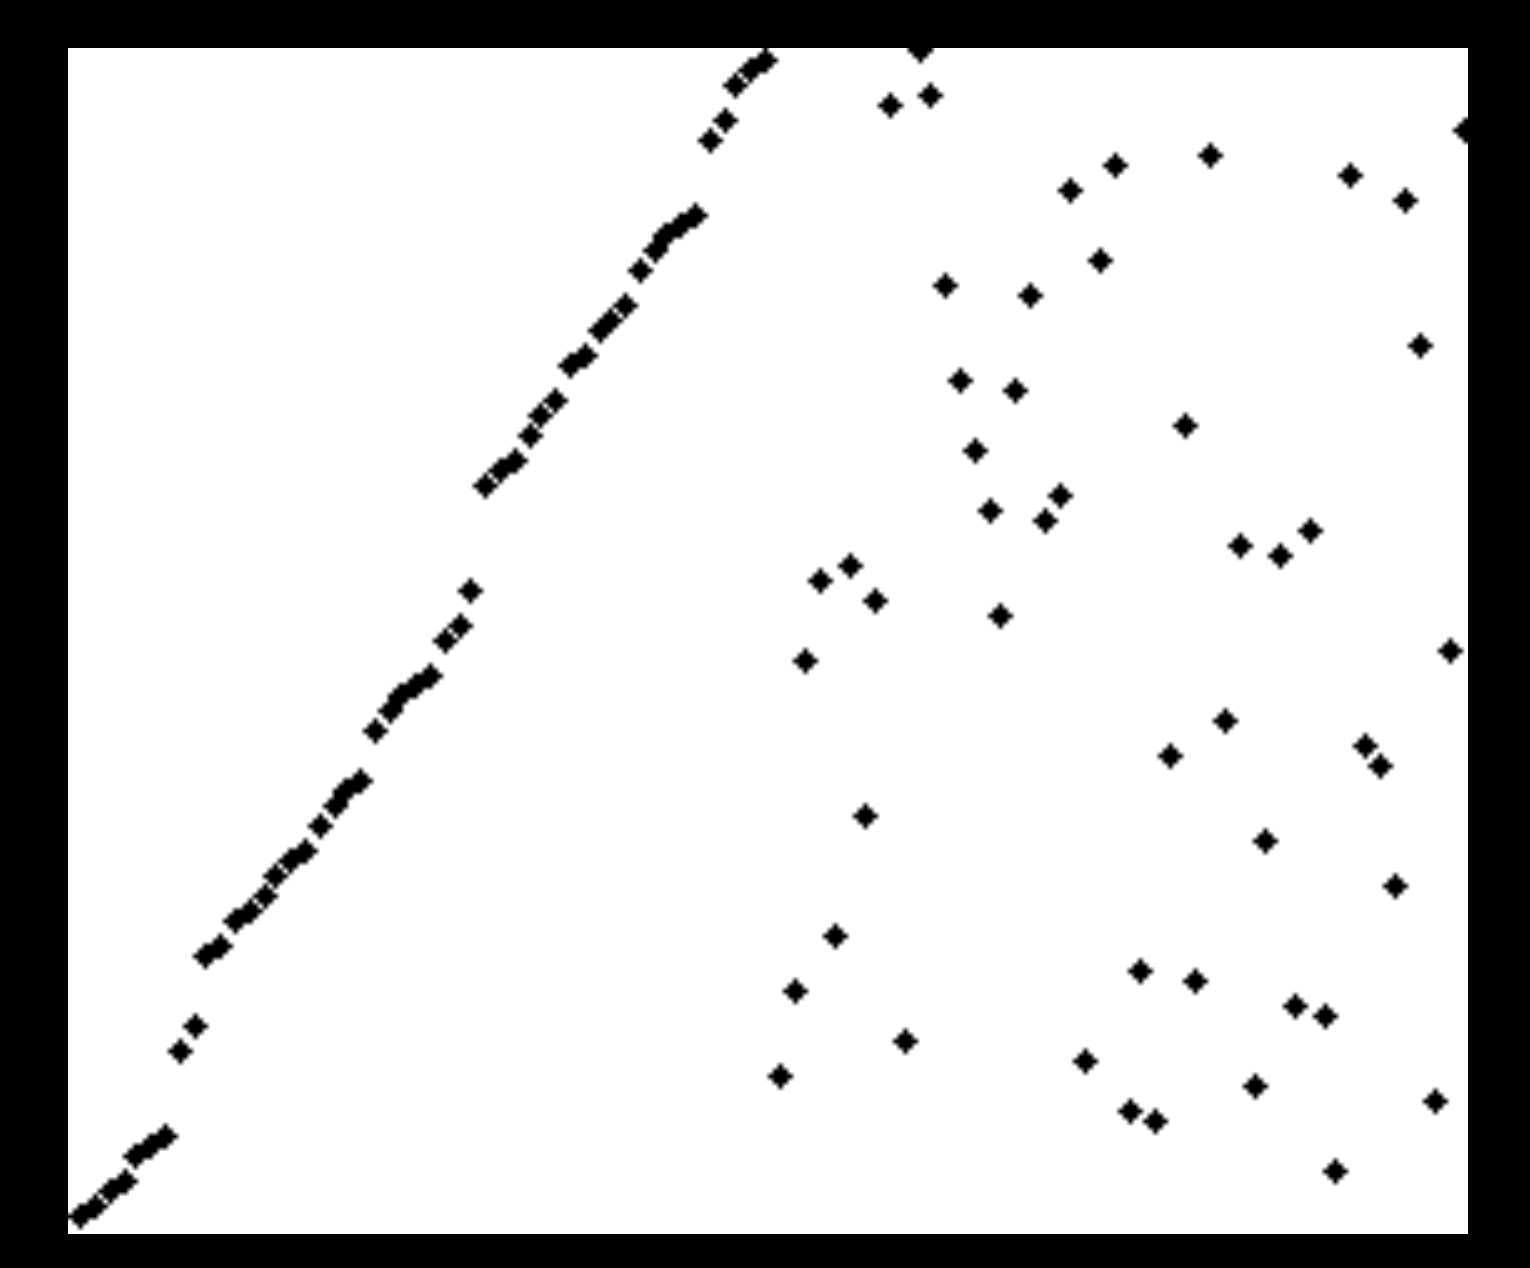
\includegraphics[width=\textwidth]{../images/msort_gif.png}

  (\href{https://upload.wikimedia.org/wikipedia/commons/c/c5/Merge_sort_animation2.gif}{animation})
\end{minipage}

\end{footnotesize}
\end{frame}

%%%%%%%%%%%%%%%%%%%%%%%%%%%%%%%%%%%%%%%%%%%%%%%%
\subsection*{Introduktion til de to eksempler}
%%%%%%%%%%%%%%%%%%%%%%%%%%%%%%%%%%%%%%%%%%%%%%%%

\begin{frame}[fragile]
\begin{footnotesize}

  \headsp{To eksempler på brug af rekursion}

  Vi skal se på brug af rekursion til to formål:

  \vspace{1ex}

  \begin{minipage}{0.5\textwidth}
  \begin{enumerate}
  \item \textbf{Implementation af spillet Towers of Hanoi.}

    \emph{Spilleren (evt. computeren) skal flytte $N$ skiver der er
      placeret i orden på den første af tre pinde til den sidste
      pind. Spilleren må kun flytte en skive af gangen og en stor
      skive må ikke placeres ovenpå en mindre.}

    \vspace{2ex}

  \item \textbf{Tegning af figurer ved hjælp af linier.}

    \emph{Ved brug af et simpelt F\# GUI interface kan vi tegne
      rekursive figurer med linier.}
  \end{enumerate}
\end{minipage}\hspace{8mm}\begin{minipage}[c]{0.4\textwidth}

\hfill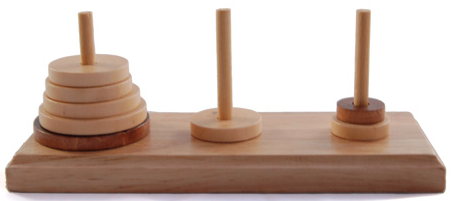
\includegraphics[width=0.9\textwidth]{../images/towersofhanoi.png}

\vspace{1ex}

\mbox{ }\hfill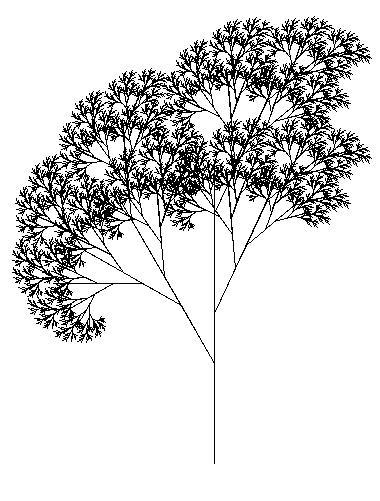
\includegraphics[width=0.6\textwidth]{../images/RecursiveTree.JPG}
\end{minipage}

\end{footnotesize}
\end{frame}

\subsection{Towers of Hanoi}
\begin{frame}[fragile]
\begin{footnotesize}

  \head{Spillet Towers of Hanoi}

  \vspace{1ex}

  \begin{minipage}[b]{0.55\textwidth}
  \begin{itemize}
  \item Spillet spilles med $N$ skiver der kan placeres på tre
    pinde.
    \vspace{1ex}

  \item Udgangspunktet er at alle skiverne ligger i orden på den
    første pind.
    \vspace{1ex}

  \item Spilleren (evt. computeren) skal flytte skiverne (en af gangen)
    således at alle ender på den fjerneste pind.
    \vspace{1ex}

\item På intet tidspunkt må en stor skive ligge ovenpå en mindre
  skive.
  \end{itemize}
\end{minipage}\hfill\begin{minipage}[b]{0.4\textwidth}

\begin{tiny}
\begin{verbatim}
     |           |           |
    ===          |           |
   =====         |           |
  =======        |           |
 =========       |           |
------------------------------------
\end{verbatim}

\begin{verbatim}
     |           |           |
     |           |           |
     |           |           |
     |           |          ===
 =========    =======      =====
------------------------------------
\end{verbatim}

\begin{verbatim}
     |           |           |
     |           |          ===
     |           |         =====
     |           |        =======
     |           |       =========
------------------------------------
\end{verbatim}
\end{tiny}
\end{minipage}
\end{footnotesize}
\end{frame}

\begin{frame}[fragile]
\begin{footnotesize}

  \head{Vi deler spillet Towers of Hanoi i to dele:}
  \vspace{1ex}

  \begin{enumerate}
  \item Et modul der implementerer spilkonfigurering og tegning af pinde og skiver.

    \emph{Dette modul vil håndhæve reglerne og give både dig og computeren mulighed for at spille.}

    \vspace{1ex}
  \item En applikation der kan spille spillet ved brug af en \textbf{rekursiv} algoritme.
  \end{enumerate}

\end{footnotesize}
\end{frame}

\begin{frame}[fragile]
\begin{footnotesize}

  \head{Modulet \lstinline{Pegs} -- (\texttt{pegs.fsi})}
  \vspace{1ex}

\begin{lstlisting}[numbers=none,frame=none,mathescape]
module Pegs

type t
val init     : int -> t
val move     : int -> int -> t -> t
val toString : t -> string

module App =
  val reset : int -> unit
  val mv    : int -> int -> unit
\end{lstlisting}

\vspace{1ex}
  \head{Bemærk:}
\begin{itemize}
\item Typen \lstinline{t} refererer til den interne repræsentation af ``spil-konfigurationen'' (skiverne på pindene).
\item Ved at ``gemme'' repræsentationen kan en bruger kun ændre på
  konfigurationen ved brug af \lstinline{init} og \lstinline{move}.
\item Modulet \lstinline{App} bruges når et menneske skal spille spillet i \verb+fsharpi+.
\end{itemize}

\end{footnotesize}
\end{frame}

\begin{frame}[fragile]
\begin{footnotesize}

  \head{DEMO af modulet \lstinline{Pegs}}
  \vspace{1ex}

\begin{verbatim}
bash-3.2$ fsharpc --nologo -a pegs.fsi pegs.fs
bash-3.2$ fsharpi --nologo -r pegs.dll --readline-

> open Pegs.App;;
> reset 3;;

    |         |         |
   ===        |         |
  =====       |         |
 =======      |         |
------------------------------

val it : unit = ()

>
\end{verbatim}

\end{footnotesize}
\end{frame}

\begin{frame}[fragile]
\begin{footnotesize}

  \head{Den interne spil-repræsentation}
  \vspace{1ex}

  \begin{itemize}
  \item Typen \lstinline{t} i \lstinline{Pegs} modulet er internt
    repræsentereret som en liste (af længde 3) af heltalslister.
  \vspace{1ex}

  \item Som eksempel kan en start-konfiguration være repræsenteret som:
\begin{lstlisting}[numbers=none,frame=none,mathescape]
  [[1;2;3];[];[]]
\end{lstlisting}
  \vspace{1ex}

\item Operationen \lstinline{Pegs.move} flytter det øverste tal i en
  liste til en anden hvis reglerne er opfyldt. Ellers \emph{fejler}
  operationen.
\begin{lstlisting}[numbers=none,frame=none,mathescape]
  val move : int -> int -> t -> t
\end{lstlisting}
  \vspace{1ex}

\item Operationen \lstinline{Pegs.init} konstruerer en ny
  start-konfiguration.
\begin{lstlisting}[numbers=none,frame=none,mathescape]
  val init : int -> t
\end{lstlisting}
  \vspace{1ex}

\item Operationen \lstinline{Pegs.toString} konstruerer en
  streng-repræsentation af en konfiguration (til udskrivning).
\begin{lstlisting}[numbers=none,frame=none,mathescape]
  val toString : t -> string
\end{lstlisting}
  \end{itemize}
\end{footnotesize}
\end{frame}

\begin{frame}[fragile]
\begin{footnotesize}

  \head{Hanoi algoritmen}
  \vspace{1ex}

  Kan vi finde en generel strategi for at gennemføre spillet uden at
  bryde reglerne?

    \vspace{1ex}

  \head{Ja --- Her er en strategi:}

    \emph{For at flytte $N$ skiver fra en \emph{startpind} til en \emph{målpind}, ved brug af en \emph{reservepind}:}

    \vspace{1ex}

  \begin{minipage}[b]{0.55\textwidth}
  \begin{itemize}
  \item Hvis $N$ er $0$: du er færdig!
  \vspace{1ex}

\item Ellers:
  \begin{enumerate}
  \item Flyt (rekursivt) $N-1$ skiver fra startpinden til reservepinden (med brug af målpinden som reservepind).
  \item Flyt 1 skive fra startpinden til målpinden.
  \item Flyt (rekursivt) $N-1$ skiver fra reservepinden til målpinden (med brug af startpinden som reservepind).
    \end{enumerate}
  \end{itemize}
\end{minipage}\hfill\begin{minipage}[b]{0.4\textwidth}

\begin{tiny}
\begin{verbatim}
     |           |           |
    ===          |           |
   =====         |           |
  =======        |           |
 =========       |           |
------------------------------------
\end{verbatim}

\begin{verbatim}
     |           |           |
     |           |           |
     |          ===          |
     |         =====         |
 =========    =======        |
------------------------------------
\end{verbatim}
\end{tiny}
\end{minipage}

\end{footnotesize}
\end{frame}


\begin{frame}[fragile]
\begin{footnotesize}

  \head{Hanoi algoritmen i F\# (\lstinline{hanoi.fs})}
  \vspace{1ex}

\begin{lstlisting}[numbers=none,frame=none,mathescape]
let rec hanoi n src aux tgt pegs =
  if n = 0 then pegs
  else let pegs = hanoi (n-1) src tgt aux pegs
       let pegs = Pegs.move src tgt pegs
       do printf "%s" (Pegs.toString pegs)
       let pegs = hanoi (n-1) aux src tgt pegs
       in pegs

let play i =
  let pegs = Pegs.init i
  do printf "%s" (Pegs.toString pegs)
  hanoi i 0 1 2 pegs

let res = play 4
\end{lstlisting}

\head{Spørgsmål:}
\begin{itemize}
\item Vi udskriver konfigurationen efter hver flytning.
\item Kan vi skrive en simpel funktion til beregning af antal flytninger?
\end{itemize}
\end{footnotesize}
\end{frame}

\begin{frame}[fragile]
\begin{footnotesize}

  \head{Simpel funktion til beregning af antal flytninger:}
  \vspace{1ex}

\begin{lstlisting}[numbers=none,frame=none,mathescape]
  let rec hanoi_count n =
    if n <= 0 then 0
    else 2*hanoi_count (n-1) + 1
  do printf "%d\n" (hanoi_count 5)
\end{lstlisting}

  \vspace{1ex}

  \head{Bemærk:}
\begin{itemize}
\item
  Funktionen \lstinline{hanoi_count} $n$ beregner tallet $2^n - 1$.
  \item Kodefilerne for \lstinline{pegs.fsi} samt \lstinline{pegs.fs}
    er tilgængelige på Absalon (under Filer).

\begin{verbatim}
bash-3.2$ fsharpc --nologo -a pegs.fsi pegs.fs
bash-3.2$ fsharpc --nologo -r pegs.dll hanoi.fs
bash-3.2$ mono hanoi.exe
...
\end{verbatim}
    \end{itemize}
\end{footnotesize}
\end{frame}

\subsection{Liniegrafik}

\begin{frame}[fragile]
\begin{footnotesize}

  \headsp{Simpel funktionalitet til Liniegrafik:}

  Biblioteket \lstinline{img_util.dll} giver mulighed for at åbne en
  simpel GUI applikation indeholdende et canvas der kan tegnes i.

  \vspace{1ex}
  Biblioteksfilerne \fbox{\lstinline{img_util.fsi}} samt
  \fbox{\lstinline{img_util.fs}} er tilgængelige via
  \url{https://github.com/diku-dk/img-util-fs}

  \vspace{1ex}

  \hspace{.75\textwidth}\fbox{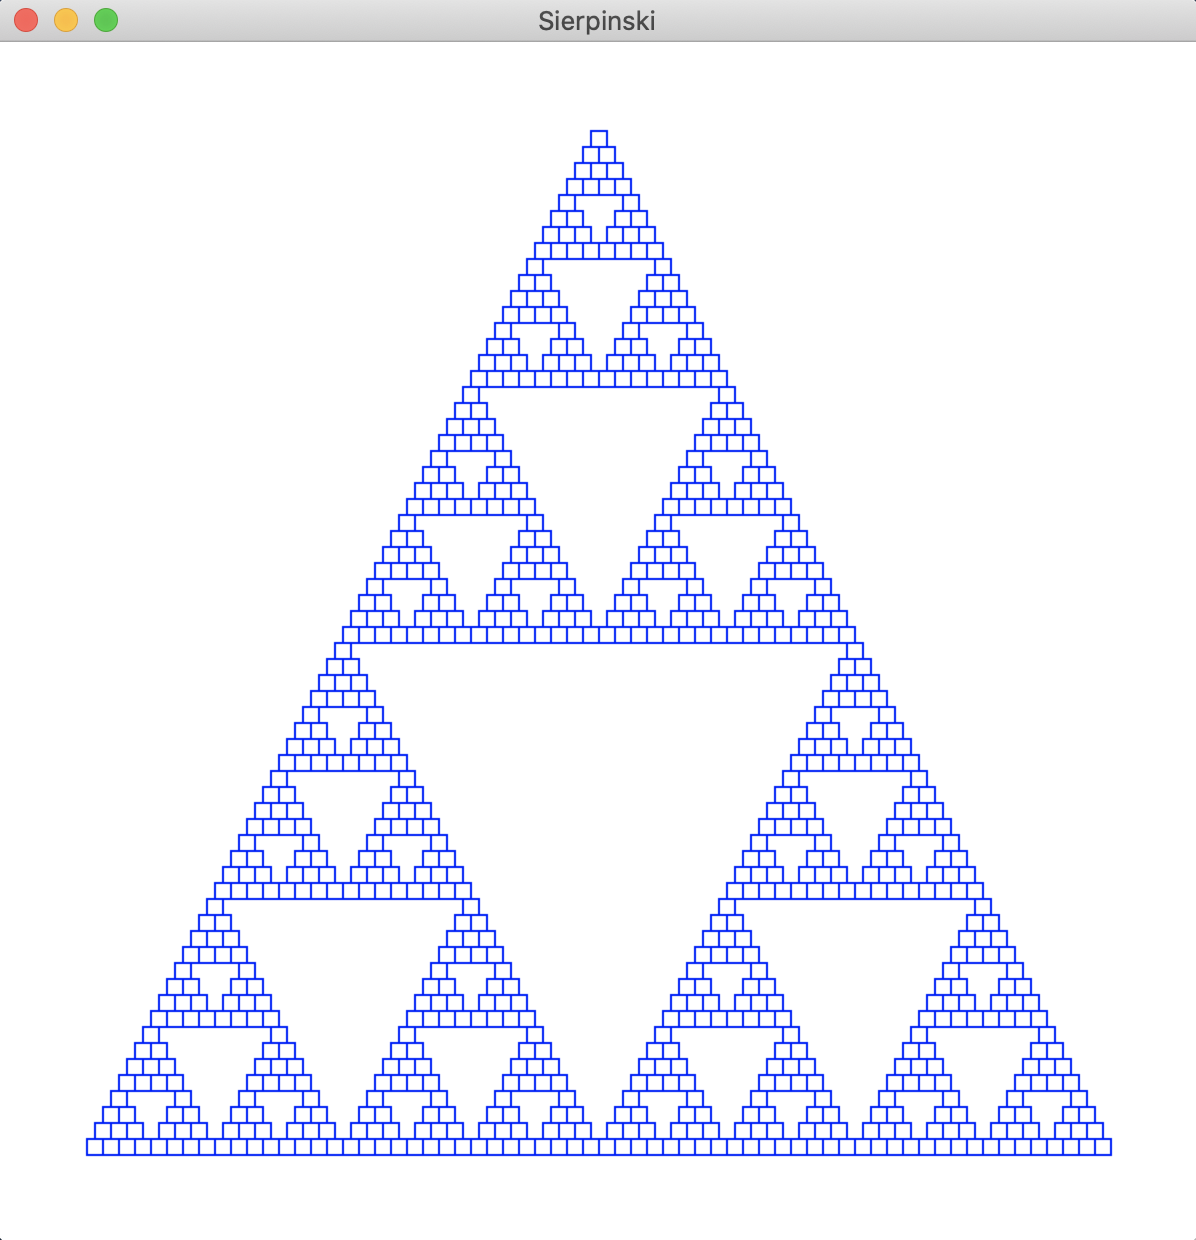
\includegraphics[width=0.2\textwidth]{../images/sierpinski_blue.png}}

  \vspace{-28mm}
  \headsp{Udvalgte funktioner (\lstinline{img_util.fsi})}

\begin{lstlisting}[numbers=none,frame=none,mathescape]
module ImgUtil

type color
val red : color

type canvas
val setLine : color -> int*int -> int*int -> canvas -> unit

val runSimpleApp : string -> int -> int
                -> (int -> int -> canvas) -> unit
...
\end{lstlisting}

\end{footnotesize}
\end{frame}

\begin{frame}[fragile]
\begin{footnotesize}

  \head{Canvas Koordinater}

  \vspace{1ex}

  Origin $(0,0)$ findes i øverste venstre hjørne.
  \vspace{1ex}

  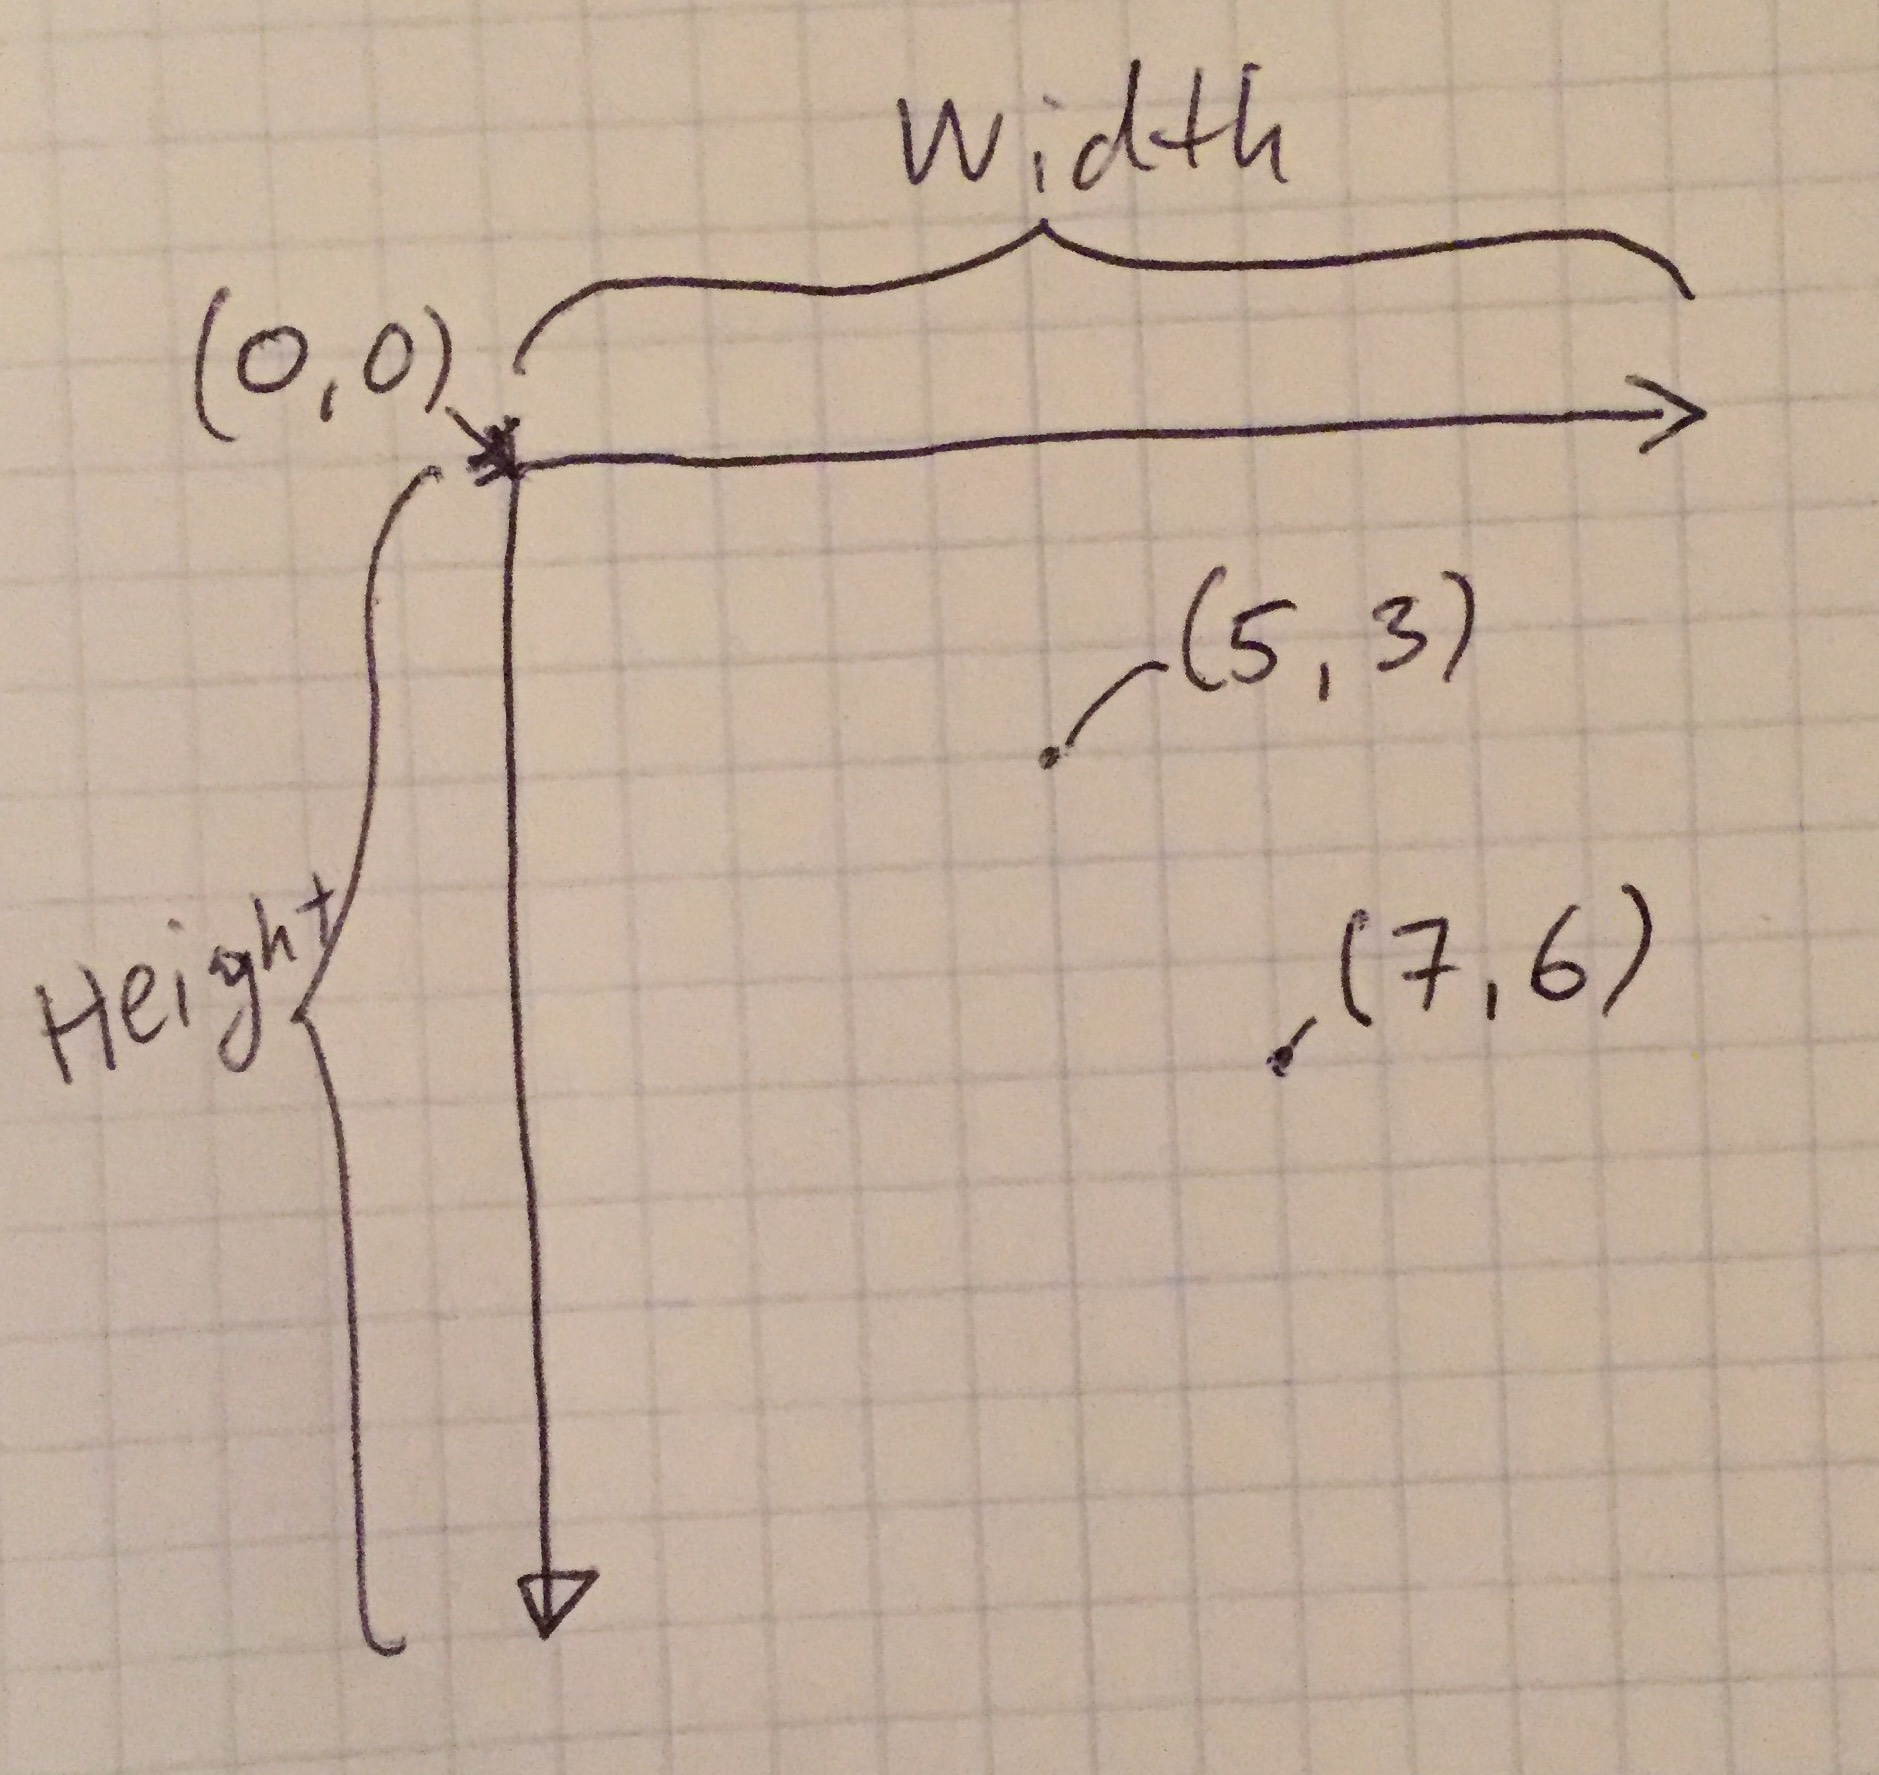
\includegraphics[width=0.6\textwidth]{../images/bitmap_coordinates.jpg}

\end{footnotesize}
\end{frame}


\begin{frame}[fragile]
\begin{footnotesize}

  \head{En simpel applikation}
  \vspace{1ex}

  \begin{minipage}[b]{0.55\textwidth}
  \begin{itemize}
  \item Konstruer en applikation med et $600\times600$ canvas.
  \vspace{1ex}

  \item Tegn en rød firkant-spiral.
  \vspace{1ex}

  \item Benyt \lstinline{setLine} funktionaliteten.
  \vspace{1ex}
  \item Start spiralen i punkt $(300,300)$
  \end{itemize}
  \end{minipage}\hfill\begin{minipage}[b]{0.4\textwidth}

  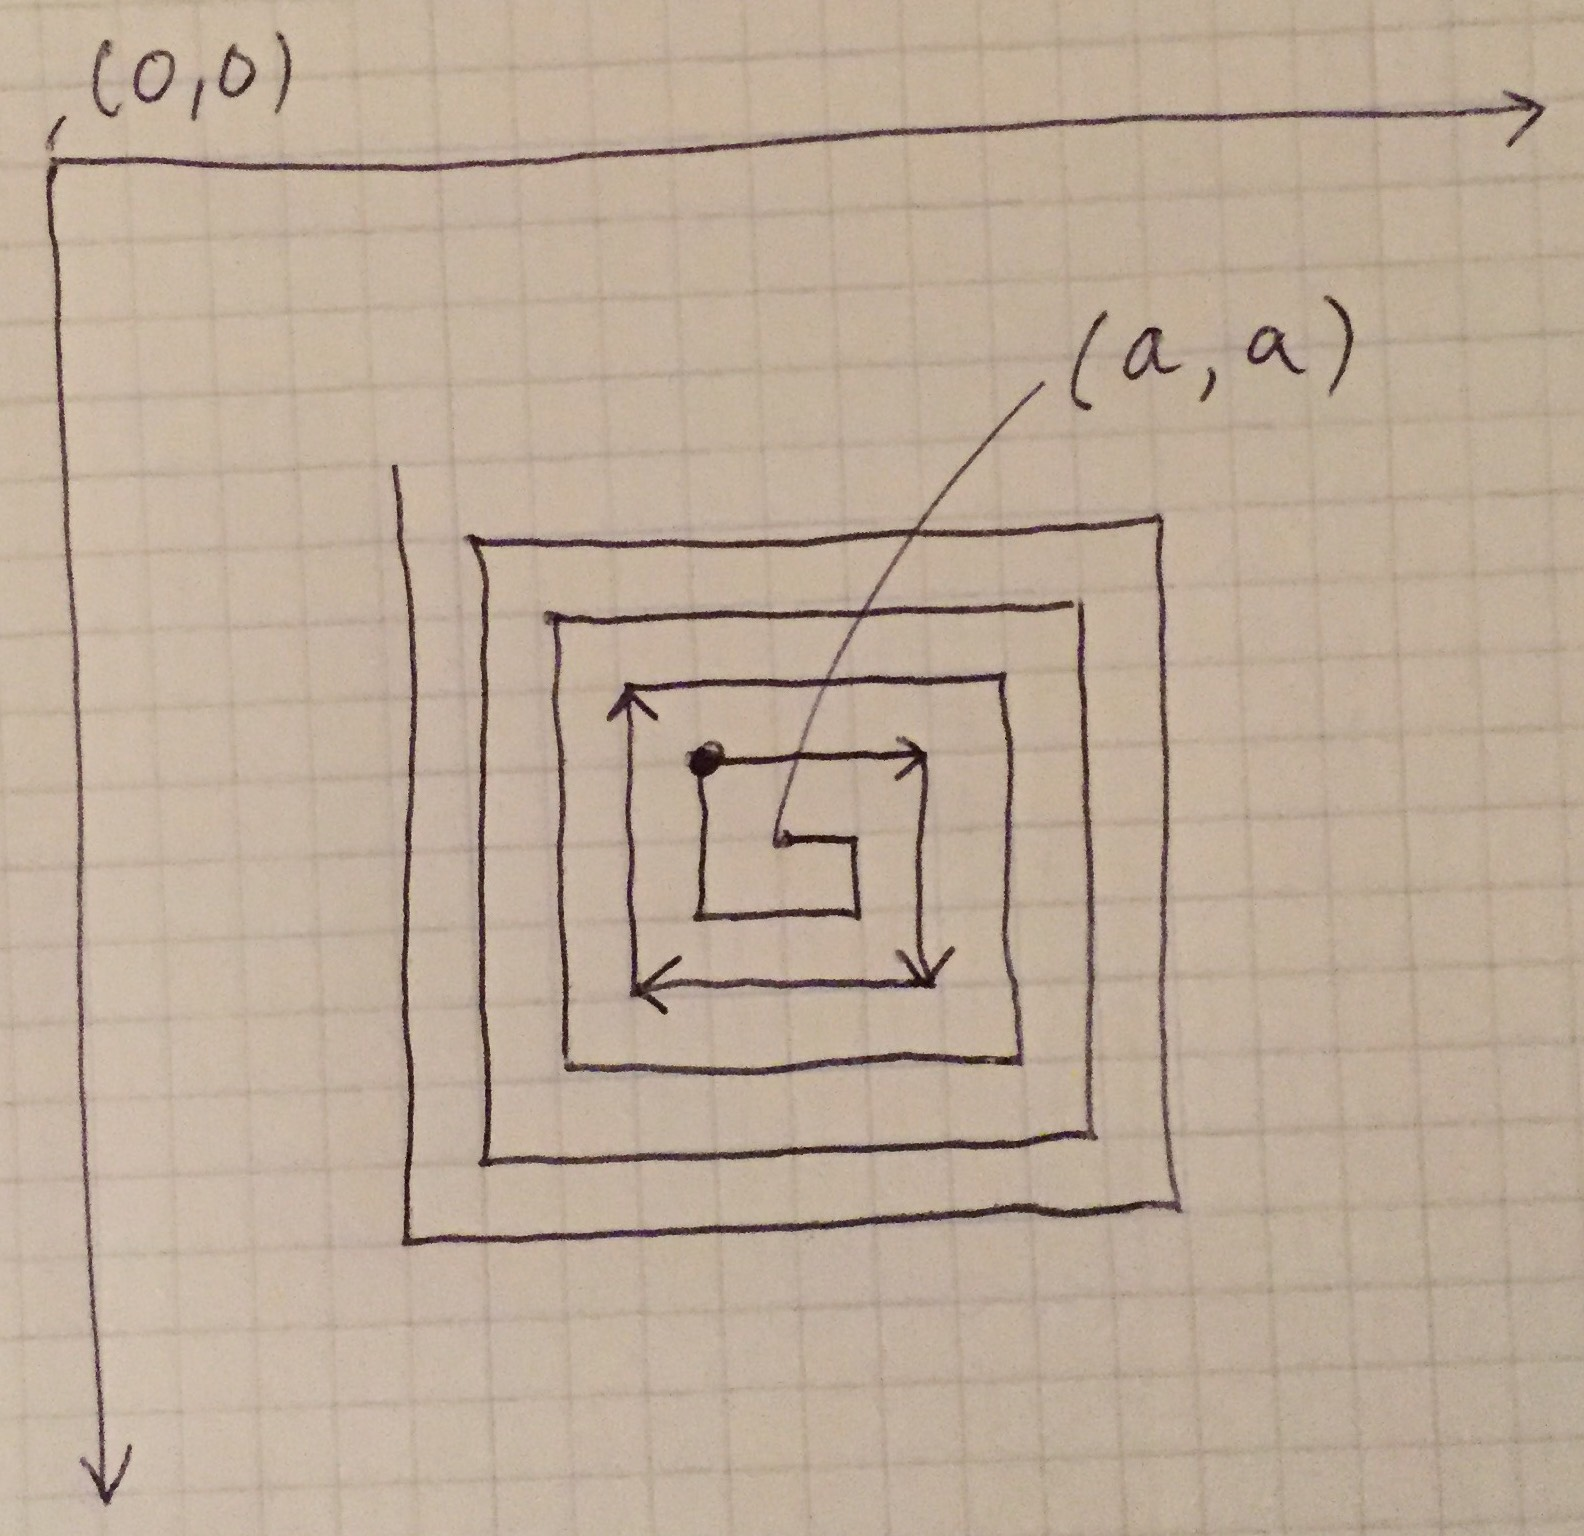
\includegraphics[width=\textwidth]{../images/spiral.jpg}
  \end{minipage}

\end{footnotesize}
\end{frame}

\begin{frame}[fragile]
\begin{footnotesize}

  \head{Koden for \lstinline{spiral.fs}}
  \vspace{1ex}

  \begin{minipage}[b]{0.65\textwidth}
\begin{lstlisting}[numbers=none,frame=none,mathescape]
open ImgUtil

let rec spiral C s i x y =
  if i >= 350 then ()
  else let p1 = (x,y)
       let p2 = (x+i,y)
       let p3 = (x+i,y+i)
       let p4 = (x-s,y+i)
       let p5 = (x-s,y-s)
       do setLine red p1 p2 C
       do setLine red p2 p3 C
       do setLine red p3 p4 C
       do setLine red p4 p5 C
       spiral C s (i+2*s) (x-s) (y-s)

let C = mk 400 400
do spiral C 10 10 200 200
do show "Spiral" C
\end{lstlisting}
  \end{minipage}\hfill\begin{minipage}[b]{0.3\textwidth}

  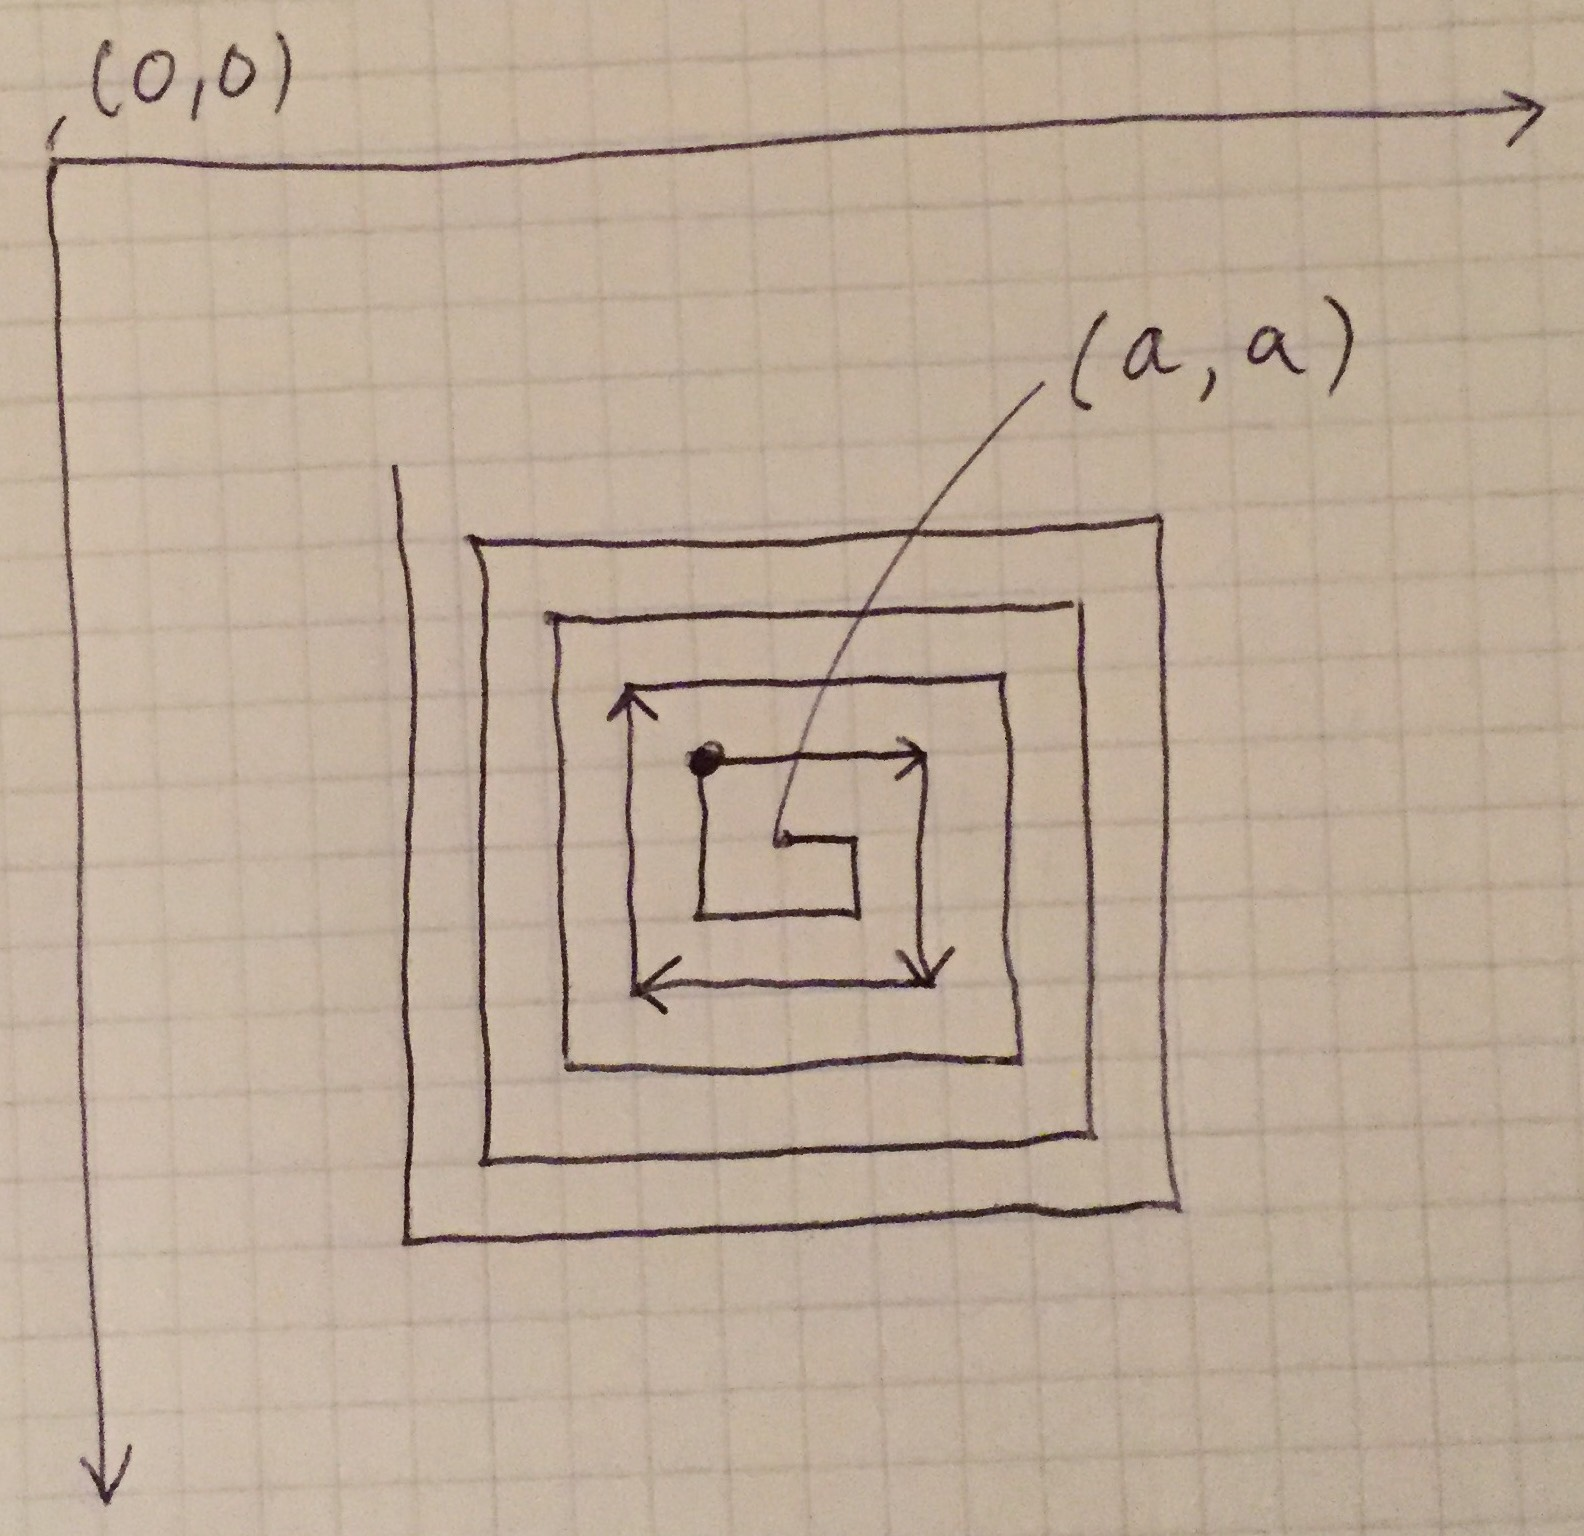
\includegraphics[width=\textwidth]{../images/spiral.jpg}

  \vspace{3cm}
  \end{minipage}

\end{footnotesize}
\end{frame}

\begin{frame}[fragile]
\begin{footnotesize}

  \head{Compil\'er og kør}
  \vspace{1ex}

  \begin{minipage}[b]{0.60\textwidth}
\begin{verbatim}
$ fsharpc -a img_util.fsi img_util.fs
$ fsharpc -r img_util.dll spiral.fs
$ mono spiral.exe
\end{verbatim}

\head{Bemærk:}
\begin{itemize}
\item Applikationen kan lukkes med ESC, f.eks.
\end{itemize}
\end{minipage}\hfill\begin{minipage}[b]{0.35\textwidth}

  \fbox{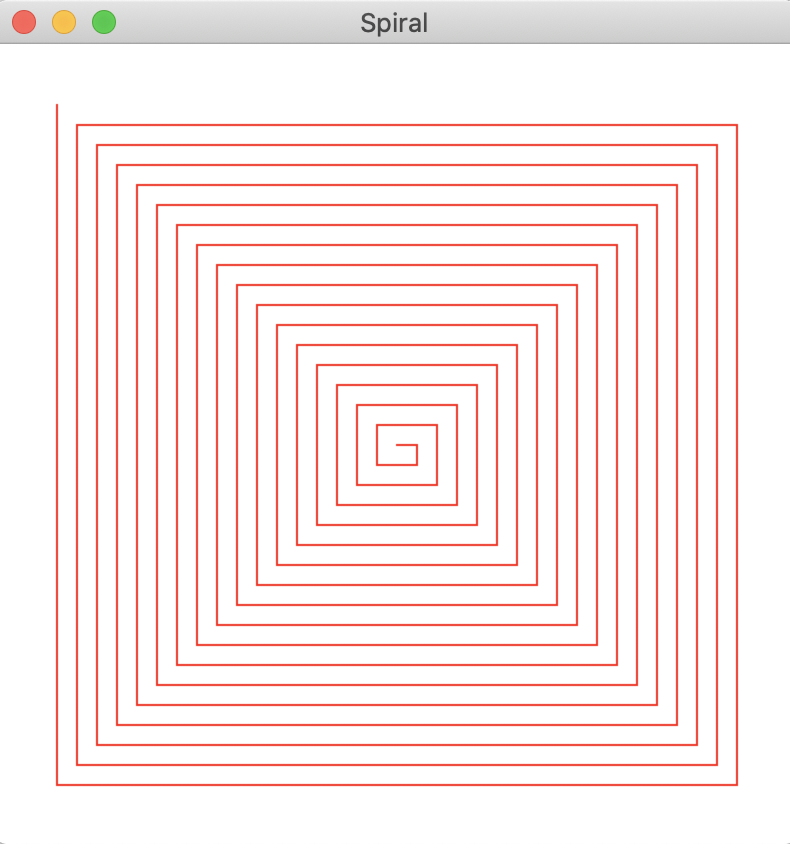
\includegraphics[width=\textwidth]{../images/spiral_red.png}}
  \end{minipage}

\end{footnotesize}
\end{frame}

\begin{frame}[fragile]
\begin{footnotesize}

  ~~\hfill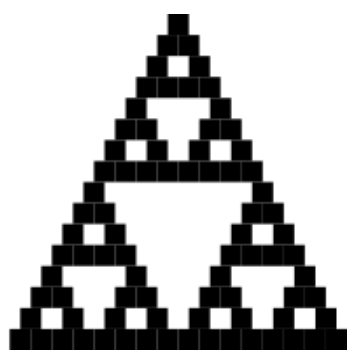
\includegraphics[width=0.2\textwidth]{../images/square_triangle.png}

  \vspace{-2.3cm}

  \head{Sierpinski --- tegn trekanter med firkanter!}

  (\texttt{sierpienski.fs})

  \head{Kode:}
\begin{lstlisting}[numbers=none,frame=none,mathescape]
open ImgUtil

let rec triangle C len (x,y) =
  if len < 12 then setBox blue (x,y) (x+len,y+len) C
  else let half = len / 2
       do triangle C half (x+half/2,y)
       do triangle C half (x,y+half)
       do triangle C half (x+half,y+half)

do runSimpleApp "Sierpinski" 600 600
      (fun w h -> let C = mk w h
                  in triangle C 512 (44,44); C)
\end{lstlisting}

\head{Compile and run:}

\begin{verbatim}
$ fsharpc -r img_util.dll sierpinski.fs
$ mono sierpinski.exe
\end{verbatim}

\end{footnotesize}
\end{frame}

\begin{frame}[fragile]
\begin{footnotesize}

  \begin{center}
  \fbox{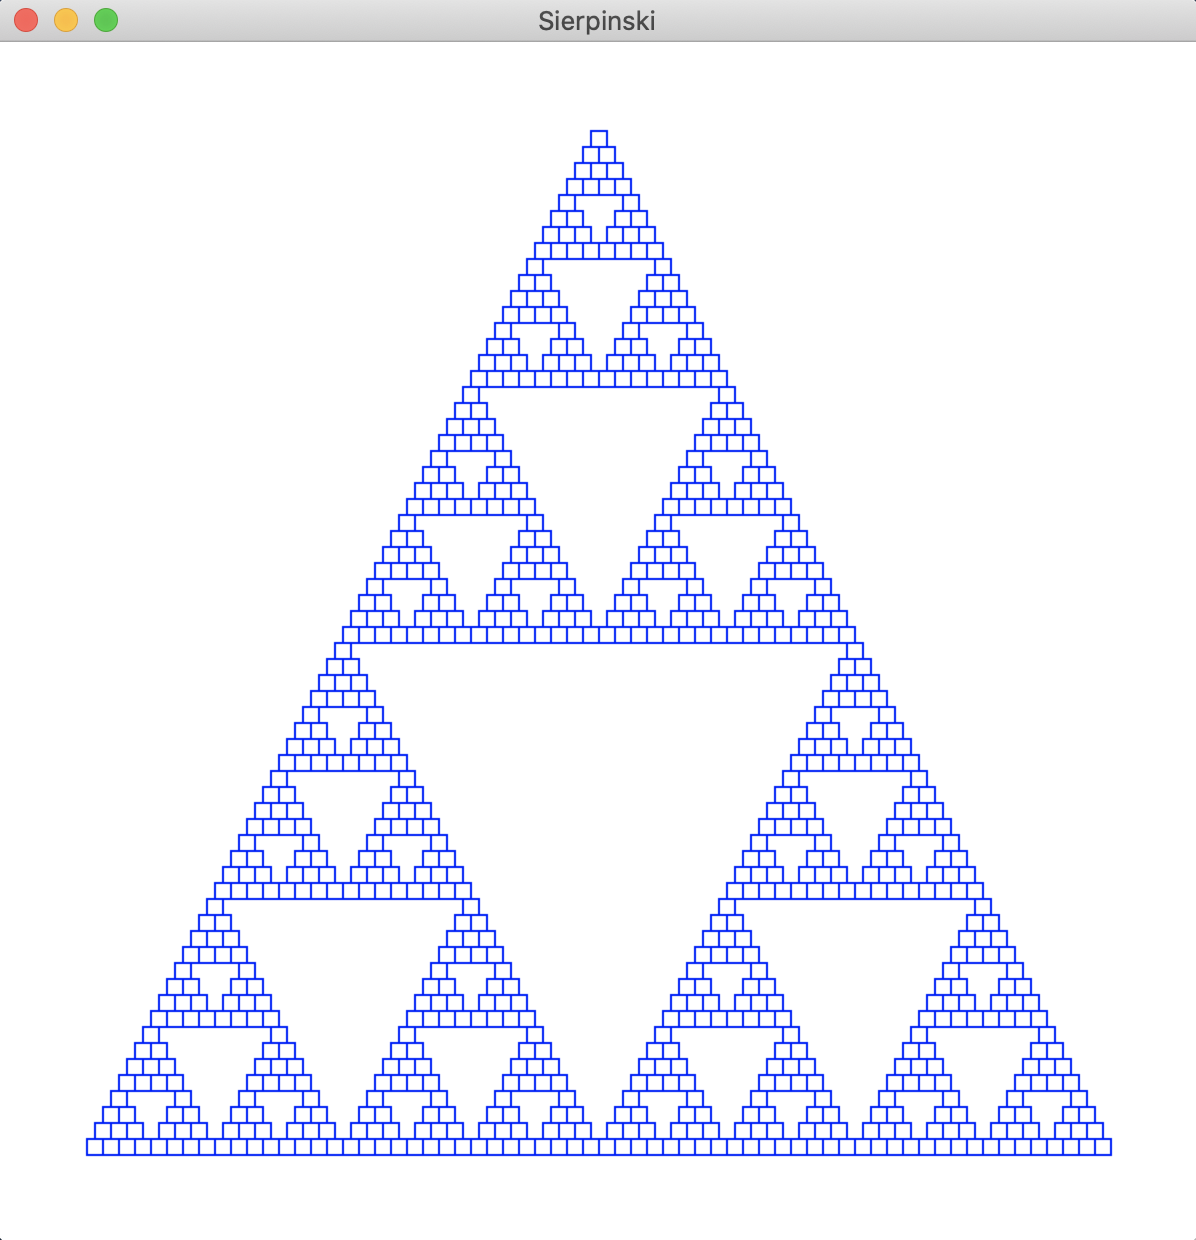
\includegraphics[width=0.6\textwidth]{../images/sierpinski_blue.png}}
  \end{center}
\end{footnotesize}
\end{frame}

\end{document}
